\clearpage
\section{Quantum Noise}

\begin{tcolorbox}	
\begin{tabular}{p{2.75cm} p{0.2cm} p{10.5cm}}
\textbf{Student Name}  &:& Diamantino Silva\\
\textbf{Starting Date} &:& October 19, 2017\\
\textbf{Goal}          &:& Simulation of quantum noise in double homodyne detection.
\end{tabular}
\end{tcolorbox}


\subsection*{Introduction}\label{sec:intro}


This document describes an emission and detection system which is used to simulate the effects of quantum noise. The system is based on the transmission of coherent states as the support of information. The following section introduces some aspects about coherent states, with special focus on quantum noise.\\
\\
\\
We start by defining number states $\ket{n}$ (or Fock states), which correspond to states with perfectly fixed number of photons.
%\footnote{Loundon, p.184}
\cite{loudon2000}
Associated to those states are two operators, the creation $\hat{a}^\dagger$ and annihilation $\hat{a}$ operators, which in a simple way, remove or add one photon from a given number state.
%\footnote{Mark Fox, p.155}
\cite{fox2006}
Their action is defined as:
\begin{equation}
\hat{a} \ket{n} = \sqrt{n} \ket{n-1}
\qquad \qquad
\hat{a}^\dagger \ket{n} = \sqrt{n+1} \ket{n+1}
\qquad \qquad
\hat{n} \ket{n} = n \ket{n}
\end{equation}
in which $\hat{n} = \hat{a}^\dagger\hat{a}$ is the number operator. Therefore, number states are eigenvectors of the number operator.\\
\\
Coherent states have properties that closely resemble classical electromagnetic waves, and are generated by single-mode lasers well above the threshold.
%\footnote{Loudon, p.190}
\cite{loudon2000}
We can defined them, using number states in the following manner:
\begin{equation}
\ket{\alpha} = e^{-\frac{|\alpha|^2}{2}} \sum_{n=0}^\infty \frac{\alpha^n}{\sqrt{n!}} \ket{n}
\end{equation}
in which the complex number $\alpha$ is the sole parameter that characterizes it.
%\footnote{Loudon, p.184}
%\footnote{Loudon, p.186}
In fact, if we calculate the expected number of photons with $\bra{\alpha} \hat{n} \ket{\alpha}$ we will obtain $|\alpha|^2$. The coherent state is an eigenstate of the annihilation operator, $\hat{a}\ket{\alpha} = \alpha \ket{\alpha}$.\\
\\
%
%
Using the creation and annihilation operators, we can define two quadrature operators:
%\footnote{Loudon, p.138, (4.3.36)}
\cite{loudon2000}
%
\begin{equation}
\hat{X} = \frac{1}{2} \left( \hat{a}^\dagger + \hat{a} \right)
\qquad
\qquad
\hat{Y} = \frac{i}{2} \left( \hat{a}^\dagger - \hat{a} \right)
\end{equation}
%
The expected value of these two operators, using a coherent state $\ket{\alpha}$ are:
%
\begin{equation}
\braket{\hat{X}} = \textrm{Re}(\alpha) \qquad \qquad
\braket{\hat{Y}} = \textrm{Im}(\alpha)
\end{equation}
%
We see that the expected value of these operators give us the real and imaginary part of $\alpha$. Now, we can obtain the uncertainty of these operators, using:
%
\begin{equation}
\textrm{Var}(\hat{X}) = \braket{\hat{X}^2} - \braket{\hat{X}}^2
\end{equation}
%
For each of these quadrature operators the variance will be:
%
\begin{equation}
\textrm{Var}(\hat{X}) = \textrm{Var}(\hat{Y}) = \frac{1}{4}
\end{equation}
%
This result show us that for both quadratures, the variance of measurement is the same and independent of the value of $\alpha$.
%
%
%
\subsubsection{Homodyne detection}
The balanced homododyne technique is used to measure the phase of the input signal (S), relative to the phase of a local oscillator (LO), which has the same frequency as the input signal, but a much larger amplitude. The technique consists in combining the input signal and the local oscillator, using a 50:50 beam splitter, from whom two beams emerge, which are then converted to currents using photodides. Finally, the two currents are subtracted, resulting in an output current.\\
A phase of the local oscillator can be defined as the reference phase. A phase offset equal to $0$ or $pi/2$ will give an output proportional to the signal's in-phase component or to the quadrature component, respectively. Therefore, the $\hat{X}$ operator will correspond to the in-phase component and $\hat{Y}$ operator correspond to quadrature component.
%\footnote{Mark Fox, p. 140}
\cite{fox2006}
\\
In the lab and in our simulations, we will use a more complex system, the double balanced homodyne detection, which allows the simultaneous measurement of the in-phase and quadrature components. The signal is divided in two beam with half the power of the original. One of the beams will be used in a balanced homodyne detection with a local oscillator. The other beam will be used in another balanced homodyne detection, but using a local oscillator with a phase difference $\pi/2$ relative to the first one.
%
\begin{figure}[H]
\label{fig:scheme_homodyne}
\centering
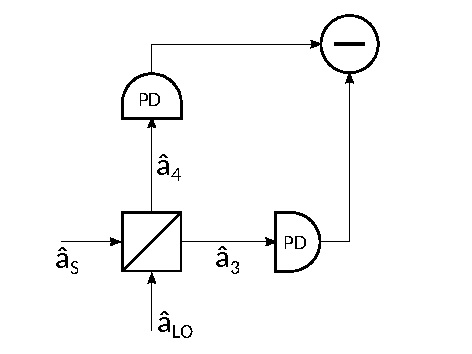
\includegraphics{./sdf/quantum_noise/figures/scheme_homodyne.pdf}
\caption{Balanced double homodyne detection.}
\end{figure}
%
%
%
\subsubsection{Noise sources in homodyne detection}
The detection of light using photodiodes is subjected to various sources of noise. One of these sources is the electrical field itself. The interaction of the signal with the vaccuum field adds quantum noise to the detection.
Another source of noise comes from the detection system, such as photodiodes and other electrical circuits, originating various kinds of noise, such as thermal noise, dark noise and amplifier noise.
%\footnote{Hans, p.185}
\cite{hans2004}
In the following sections, we will focus on two noise sources, quantum noise and thermal noise.
%
%
%
\subsubsection{Quantum Noise}
In order to grasp this effect, the quantum mechanical description of balanced homodyne detection will be used, employing quantum operators to describe the effect of each component in the system (fig. \ref{fig:scheme_homodyne}). We start with the operators $\hat{a}_S$ and $\hat{a}_{LO}$ corresponding to the annihilation operator for the signal and local oscillator, which are the inputs in a beam divisor. The outputs will be $\hat{a}_3$ and $\hat{a}_4$.
Using a balanced beam splitter, we can write the output as:
%
\begin{equation}
\hat{a}_3 = \frac{1}{\sqrt{2}} \left( \hat{a}_S + \hat{a}_{LO} \right)
\qquad
\qquad
\hat{a}_4 = \frac{1}{\sqrt{2}} \left( \hat{a}_S - \hat{a}_{LO} \right)
\end{equation}
%
The final output of a homodyne measurement will be proportional to the difference between the photocurrents in arm $3$ and $4$. Then
%
\begin{equation}
I_{34} = I_3 - I_4 \sim \braket{\hat{n}_3 - \hat{n}_4}
\end{equation}
%
We can define an operator that describes the difference of number of photons in arm 3 and arm 4:
%
\begin{equation}
\hat{m} = \hat{a}^\dagger_3\hat{a}_3 - \hat{a}^\dagger_4\hat{a}_4
\end{equation}
%
If we assume that the local oscillator produces the the coherent state $\ket{\beta}$, then the expected value of this measurement will be:
%
\begin{equation}
\label{eq:noise}
\braket{m} = 2|\alpha||\beta|\cos({\theta_\alpha - \theta_\beta})
\qquad
\qquad
\textrm{Var}(m) = |\alpha|^2 + |\beta|^2
\end{equation}
%
The local oscillator normally has a greater power than the signal
%VER REFERENCIAS
, then $|\alpha| \ll |\beta|$. If we use as unit, $2|\beta|$, then these two quantities can be simplified to:
%
\begin{equation}
\label{eq:approx_noise}
\braket{m} = |\alpha|\cos({\theta_\alpha - \theta_\beta})
\qquad
\qquad
\textrm{Var}(m) \approx \frac{1}{4}
\end{equation}
%
%\footnote{Referencia indirecta: Livro: Hans, p.207}
\cite{hans2004}
\\
Has we have seen previously, in order to measure two quadratures simultaneously, we can use double balanced homodyne detection. For each quadrature, the input signal now has half the power, so $|\alpha| \rightarrow |\alpha/\sqrt{2}|$.  If we use a local oscillator that produces states $\ket{\beta}$, then we can divide it in two beams in state $\ket{\beta/\sqrt{2}}$ and $\ket{i\beta/\sqrt{2}}$ which will be used in each homodyne detection. In this setting, the expected values for each quadrature, $X$ and $Y$, (in normalized values of $\sqrt{2}|\beta|$) are:
%
\begin{equation}
\braket{m_X} = \left|\frac{\alpha}{\sqrt{2}}\right| \cos({\theta_\alpha - \theta_\beta})
\qquad
\qquad
\textrm{Var}(m_X) \approx \frac{1}{4}
\end{equation}
%
%
\begin{equation}
\braket{m_Y} =  \left|\frac{\alpha}{\sqrt{2}}\right| \sin({\theta_\alpha - \theta_\beta})
\qquad
\qquad
\textrm{Var}(m_Y) \approx \frac{1}{4}
\end{equation}
%
Therefore the measurement of each quadrature will have half the amplitude, but the same variance.
%
%
%
\subsubsection{Thermal noise}
Thermal noise is generated by electrons in response to temperature. It's contribution to the resulting current can be described by the following equation:
%\footnote{Mark Fox, p. 96}
\cite{fox2006}
%
\begin{equation}
\braket{(\Delta i_T)^2} = 4 K_B T_0 B/R_L
\end{equation}
%
in which $K_B$ it's Boltzmann's constant, $T_0$ is the absolute temperature, $B$ is the bandwidth and $R_L$ is the receiver load impedance. The $B$ value is imposed by default or chosen when the measurements are made, but the $R_L$ value is dependent in the internal setup of the various components of the detection system. Nevertheless, for simulation purposes, we can just introduce an experimental value.\\
\vspace{1cm}
%
%
\subsection*{Simulation}

The simulation setup is represented in figure \ref{fig:setup}. The starting point is the MQAM, which generates random states from a given constelation. The output from the generator is received in the Optical Hybrid where it is mixed with a local oscillator, outputing two optical signal pairs. Each pair is converted to currents by two photodiodes, and then subtracted from each other, originating a current proportional to one of the quadratures of the input state. 
The other pair suffers the same process, but the resulting subtraction current will be proportional to another quadrature, dephased by $\pi/2$ relative to the other quadrature.\\
%
\begin{figure}[H]
\centering
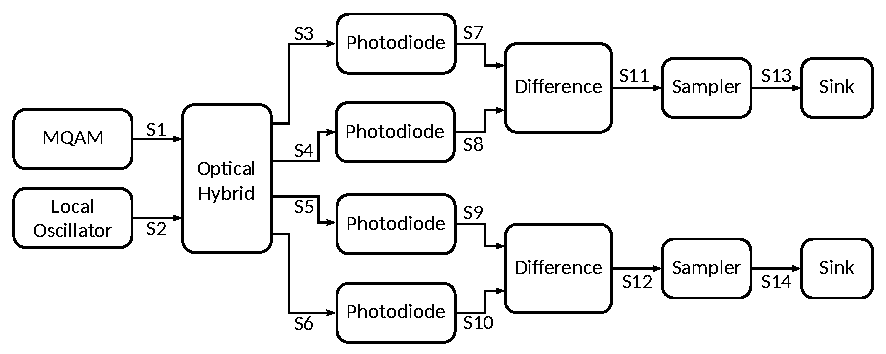
\includegraphics[width=\linewidth]{./sdf/quantum_noise/figures/scheme_setup.pdf}
\caption{Overview of the simulated optical system.}
\label{fig:setup}
\end{figure}
%
\begin{table}[H]
\centering
\begin{tabular}{c|c}
System Blocks                         & netxpto Blocks\\
\hline
M - Quadrature Amplitude Modulator    & MQamTransmitter\\
Local Oscillator                      & LocalOscillator\\
90deg Optical Hybrid                  & OpticalHybrid\\
Photodiode                            & Photodiode\\
Difference Circuit                    & Difference\\
Sampler                               & Sampler\\
\end{tabular}
\end{table}


\subsection*{Required files}\label{Required files}

Header Files
\begin{table}[H]
\centering
\begin{tabulary}{1.0\textwidth}{|L|L|}
\hline
\textbf{File}           & \textbf{Description}\\
\hline
netxpto.h               & Generic purpose simulator definitions.\\
\hline
m\_qam\_transmitter.h   & Outputs a QPSK modulated optical signal.\\
\hline
local\_oscillator.h     & Generates continuous coherent signal.\\
\hline
optical\_hybrid.h       & Mixes the two input signals into four outputs.\\
\hline
photodiode.h            & Converts an optical signal to a current.\\
\hline
difference.h            & Ouputs the difference between two input signals.\\
\hline
sampler.h               & Samples the input signal.\\
\hline
sink.h                  & Closes any unused signals.\\
\hline
\end{tabulary}
\end{table}
%
%
Source Files
\begin{table}[H]
\centering
\begin{tabulary}{1.0\textwidth}{|L|L|}
\hline
\textbf{File}                   & \textbf{Description}\\
\hline
netxpto.cpp                     & Generic purpose simulator definitions.\\
\hline
m\_qam\_transmitter.cpp         & Outputs a QPSK modulated optical signal.\\
\hline
local\_oscillator.cpp           & Generates continuous coherent signal.\\
\hline
optical\_hybrid.cpp             & Mixes the two input signals into four outputs.\\
\hline
photodiode.h                    & Converts an optical signal to a current.\\
\hline
difference.h                    & Ouputs the difference between two input signals.\\
\hline
sampler.cpp                     & Samples the input signal.\\
\hline
sink.cpp                        & Empties the signal buffer.\\
\hline
\end{tabulary}
\end{table}


\subsection*{System Input Parameters}

This system takes into account the following input parameters:
\begin{table}[H]
\centering
\begin{tabulary}{1.0\textwidth}{|C|L|}
\hline
\textbf{System Parameters} & \textbf{Description}\\
\hline
numberOfBitsGenerated   & Gives the number of bits to be simulated\\
\hline
bitPeriod               & Sets the time between adjacent bits\\
\hline
wavelength              & Sets the wavelength of the local oscillator in the MQAM\\
\hline
samplesPerSymbol        & Establishes the number of samples each bit in the string is given\\
\hline
localOscillatorPower1   & Sets the optical power, in units of W, of the local oscillator inside the MQAM\\
\hline
localOscillatorPower2   & Sets the optical power, in units of W, of the local oscillator used for Bob's measurements\\
\hline
localOscillatorPhase    & Sets the initial phase of the local oscillator used in the detection\\
\hline
transferMatrix          & Sets the transfer matrix of the beam splitter used in the homodyne detector\\
\hline
responsivity            & Sets the responsivity of the photodiodes used in the homodyne detectors\\
\hline
bufferLength            & Sets the length of the buffer used in the signals\\
\hline
iqAmplitudeValues       & Sets the amplitude of the states used in the MQAM\\
%\hline
%shotNoise (FUTURE)      & Chooses if quantum shot noise is used in the simulation\\
\hline
samplesToSkip           & Sets the number of samples to skip when writing out some of the signal files\\
%\hline
%thermalNoise (FUTURE)   & Chooses if thermal noise is used in the simulation\\
%\hline
%thermalNoiseAmplitude  (FUTURE)  & Sets the amplitude of the thermal noise\\
\hline
\end{tabulary}
\end{table}        

\subsection*{Inputs}

This system takes no inputs.

\pagebreak
\subsection*{Outputs}

The system outputs the following objects:
\begin{itemize}
\item Signals:
\begin{itemize}
\item Binary Sequence used in the MQAM; (S$_{0}$)
\item Local Oscillator used in the MQAM; (S$_{1}$)
\item Local Oscillator used in the detection; (S$_{2}$)
\item Optical Hybrid Outputs; (S$_{3}$, S$_{4}$, S$_{5}$, S$_{6}$)
\item In phase Photodiodes output; (S$_{7}$, S$_{8}$)
\item Quadrature Photodiode output; (S$_{9}$, S$_{10}$)
\item In phase Difference output; (S$_{11}$)
\item Quadrature Difference output; (S$_{12}$)
\item In phase Sampler output; (S$_{13}$)
\item Quadrature Sampler output; (S$_{14}$)
\end{itemize}
\end{itemize}    





\subsection*{Simulation Results}\label{subsec:SHresults}

To test the simulated implementation, a series of states $\{\ket{\phi_i}\}$ were generated and detected, resulting in a series of measurements $\{(x_i,y_i)\}$. The simulation result is presented in figure $\ref{fig:constelation}$:
%
\begin{figure}[H]
\centering
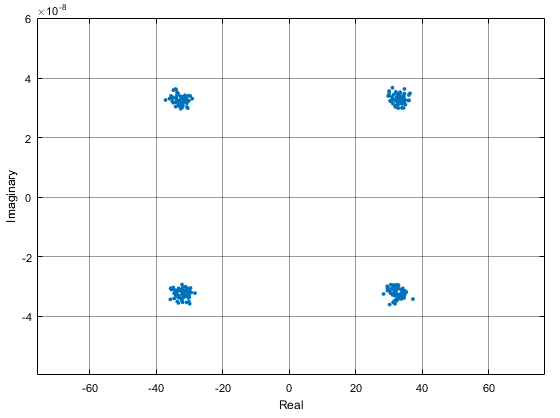
\includegraphics[width=10cm]{./sdf/quantum_noise/figures/constelation1.png}
\caption{Simulation of a constelation of 4 states (n = 100)}
\label{fig:constelation}
\end{figure}
%
We see that the measurements made groups in certain regions. Each of this groups is centered in the expected value $(\braket{\textrm{X}}, \braket{\textrm{Y}})$ of one the generated states. Also, they show some variance, which was tested for various expected number of photons, $\braket{n}$, resulting in figure \ref{fig:variance}:
%
\begin{figure}[H]
\captionsetup{justification=centering}
\centering
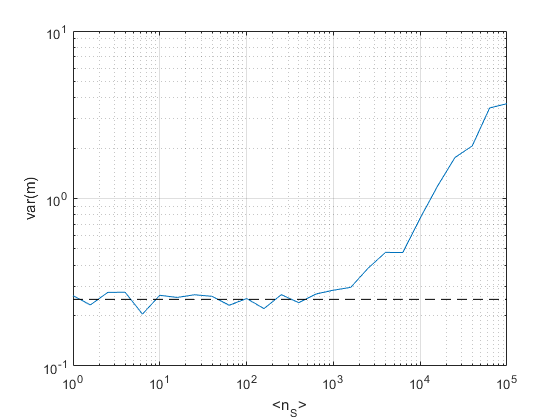
\includegraphics[width=10cm]{./sdf/quantum_noise/figures/plot_var_vs_n1.png}
\caption{Simulation of the variance of $m$.\\Local oscillator expected number of photons: $10^4$}
\label{fig:variance}
\end{figure}
%
It was expected that the variance should independent of the input's signal number of photons. Plot \ref{fig:variance} shows that for low values of $n_S$, the simulation is in accordance with the theoretical prevision, with $\textrm{Var(X)} = \textrm{Var(Y)} = \frac{1}{4}$ . For large values of $n_S$, when the number of photons is about the same has the local oscillator, the quantum noise variance starts to grow proportionally to $n_S$, in accordance with the non approximated calculation of quantum noise (eq. \ref{eq:noise}).\\
\\
{\bf Noise Variance with LO power Simulation}\\
The following plot shows the behavior of current noise variance $\braket{(\Delta i)^2}$ with local oscilator power, $P_{LO}$:
%
%
\begin{figure}[H]
\centering
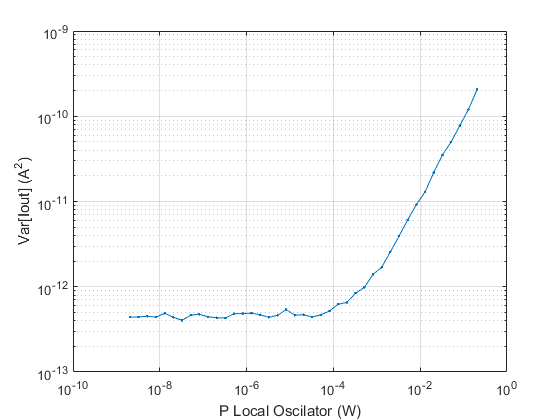
\includegraphics[width=10cm]{./sdf/quantum_noise/figures/power_plot.png}
\caption{Output current variance in function of LO power.}
\label{fig:variance_lo_power}
\end{figure}
%
%
We see that for low LO power, the dominant noise is the thermal contribution, but for higher power, quantum noise dominates, growing proportionally to $P_{LO}$. This in accordance with equation \ref{eq:approx_noise}\\
\\
\\
{\bf Comparison to experimental results}\\
As we have seen earlier, the system will manifest noise even in the absence of input signal (eq \ref{eq:noise}). The experimental procedure for this measurement consisted in just inputing the local oscillator laser and no signal. For each value of  $P_{LO}$, the local oscillator was pulsed, and for each pulse, the variance of the plateau of the maximum was calculated. The final variance was simply the mean of the variances of all pulses.
%
\begin{figure}[H]
    \begin{subfigure}{.5\textwidth}
        \centering
        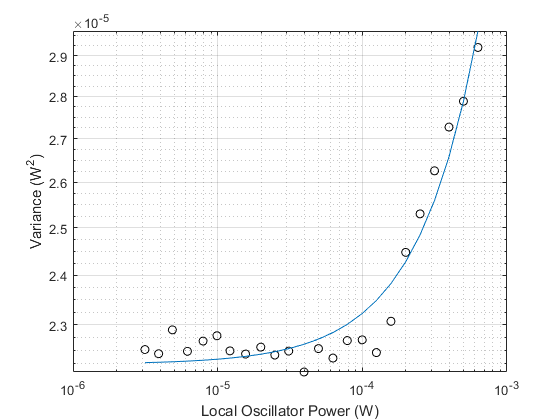
\includegraphics[width=.8\linewidth]{./sdf/quantum_noise/figures/noise_exp_channel1.png}
        \caption{$X$ quadrature}
        \label{fig:noise-exp-1}
    \end{subfigure}%
    \begin{subfigure}{.5\textwidth}
        \centering
        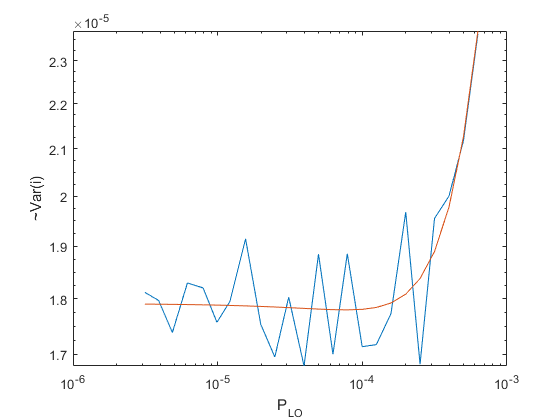
\includegraphics[width=.8\linewidth]{./sdf/quantum_noise/figures/noise_exp_channel3.png}
        \caption{$Y$ quadrature}
        \label{fig:noise-exp-3}
    \end{subfigure}
    \captionsetup{justification=centering}
    \caption{Noise variance dependency with local oscilator power for two different quadratures. Experimental vs fitted data.}
\end{figure}
%
Figures $\ref{fig:noise-exp-1}$ and $\ref{fig:noise-exp-3}$ show measures measurements of total noise for two different quadratures. For low power of LO, the noise variance flutuates around a constant value. For high power of LO, $(P_{LO}>10^{-4}W)$, the variance of noise shows an increasing trend roughly proportional to $P_{LO}^2$. The expected growth should be proportional to $P_{LO}$, but the RIN noise, originated by the electric apparatus, grows quadratically with the power, dominating the noise amplitude for large $P_{LO}$.\\
So, we see that both the simulation and experimental data display a similar behaviour, but the quadratic growth of noise for large $P_{LO}$ was not predicted in the simulations.\\
%
%



\bibliography{./sdf/quantum_noise/quantum_noise}
